% !TEX root =  ../main.tex


\begin{figure*}[t!]
\centering
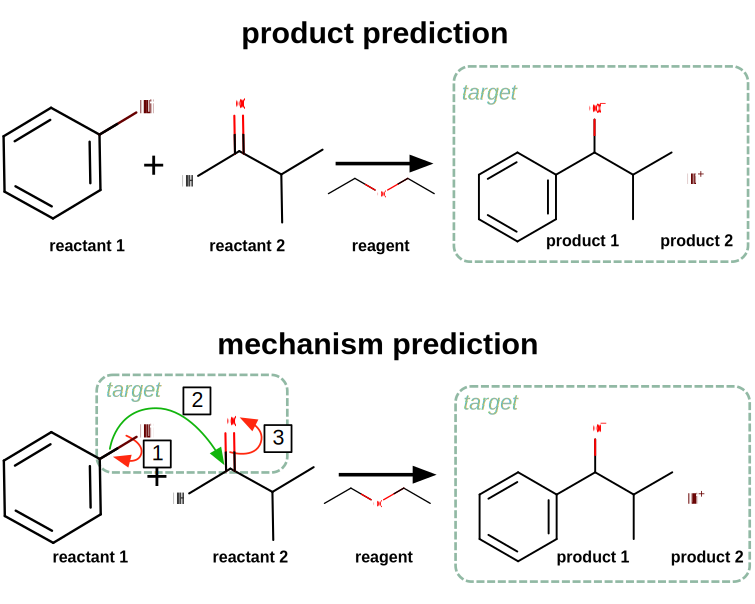
\includegraphics[width=\textwidth]{reaction_diagram}
\caption{Left: the reaction prediction problem: Given the reactants and reagents, predict the structure of the product. Right: the reaction mechanism prediction problem: Given the reactants, reagents and products, predict how the reaction occurred to form the products.}
\label{fig:task-overview}
\end{figure*}


Consider Figure \ref{fig:task-overview}. In it we show the two challenges we tackle in this paper. 
On the left we show reaction prediction; this involves predicting the reaction products, given a set of reactants and reagents. However, for this task we do not care {\em how} the reactants react.
 This job of finding the {\em how} is the target in reaction mechanism prediction, where the steps in a reaction are called a reaction mechanism.
 Before discussing how our model predicts mechanisms in the next section we use the rest of this section to describe the types of reactions we consider in this paper, and their properties.

%\todo[]{Where is the related work section going...? "And how it relates to previous work on reaction prediction. -- " }

\paragraph{Molecules and Chemical reactions.}


%In reality, the structure of a molecule is due to how electrons on each atom are interacting with each other. 
%Molecules consist of a set of atoms that are arranged into a structure by bonds, which are localized electrons. 
Molecules can be modelled as a graph structure, where each node is an atom and each edge is a covalent bond.
These covalent bonds represent the fact that 
one or more pairs of electrons are shared between the atoms that the bond connects. 


Just as electrons describe the current structure of molecules, 
they also describe how molecules react with other molecules to produce new ones. 
All chemical reactions involve the stepwise movement of electrons along the atoms in a set of reactant molecules. 
This movement causes the formation and breaking of chemical bonds that changes the reactants into a new set of product molecules.\cite{herges1994coarctate} 
In this work, we will only consider reactions with steps that involve pairs of electrons moving, and
where steps start with electron pairs on a single atom (called \emph{lone pair}), or with the electrons in an existing bond. 
These kind of reactions describe more than 80\% of \emph{organic reactions}\cite{herges1994coarctate} \footnote{Reactions that do not satisfy these assumptions are homolytic reactions, and electrocyclic reactions.}. 
Organic reactions are those involving Carbon atoms, and have a large number of applications from drug design to the invention of new materials\cite{segler2018planning}.


\paragraph{Reactions as single electron paths.}
If reactions satisfy the above restrictions, then a chemical reaction is can be modelled as pairs of electrons moving in a \emph{single path} through the reactant atoms. 
Further, this electron path will alternately remove existing bonds in molecules, and form new ones. We show this alternating structure in the right hand part of Figure \ref{fig:task-overview}. \todo[]{someone check the chemically accurateness of this.}
In this Figure, the reaction formally starts by taking the pair of electrons between the Li and C atoms and moving them to the C atom (step 1). This is a remove bond step. 
Next comes an add step where electrons are moved from the C atom to form a bond between the two reactant molecules (step 2).
Then a pair of electrons are removed between a C and O and moved to the O atom, giving rise to intermediate 1 (step 3). This will then further undergo bond making/breaking steps until the final product is formed.

Predicting the final product is thus a byproduct of predicting this series of electron steps.

However, there are a number of benefits of predicting electron paths over predicting the outcomes of reactions directly (as in previous work \cite{jin2017predicting,schwaller2017found}):
\begin{itemize}
\item \textbf{Easy to interpret}: If the model makes a mistake, it is easy to see where it goes wrong by comparing the steps of the path with the correct steps.
\item \textbf{Sparse}: Reactions often only affect between 3 and 7 atoms out of anywhere from 10-50 reactant atoms. Modeling the reaction as a path allows us to exploit this sparsity.
\item \textbf{Chemical constraints}: Learning a path allows us to easily incorporate chemical constraints, such as the alternating removal and addition of bonds, among others.
\item \textbf{Compositionally}: Learning to combine lower-level abstractions of chemistry potentially allows to generalize better.
\end{itemize}
The only other work we are aware of to use machine learning to predict reaction mechanism are the works \cite{kayala2011learning,kayala2012reactionpredictor}. However,
it relies on complex hand-coded rules and expert-annotated datasets, which are usually small and proprietary.
% Machine learning has been applied mostly for the quantum chemistry-level\cite{NIPS2012_4830,schutt2017schnet}. Additionally, various models have been proposed to predict global rewriting rules for reaction prediction\cite{coley2017prediction,jin2017predicting,neural-symbolic,schwaller2017found,wei2016neural,zhang2005structure}. These models can be trained on large sets of reported chemical reactions. 
%At the medium level of abstraction, Kayala et al. proposed a model to predict electron shift steps using of two independently learned learning-to-rank and scoring stages,
% which however relies on complex hand-coded rules and expert-annotated datasets, which are usually very small.

